\documentclass[11pt]{article}
\usepackage[margin=1in]{geometry}
\usepackage{amsmath,amssymb}
\usepackage{hyperref}
\usepackage{graphicx}

\title{Why $P_b$ and the Starlight table disagree at large $y$:\\
investigation notes}
\author{}
\date{\today}

\begin{document}
\maketitle

\section{Summary}

The photon flux computed by this code (labelled $P_b$, following the
Baur--Hencken--Trautmann point-like equivalent-photon formula used in our
paper's Eq.~(2)) disagrees with Petja Paakkinen's tabulated ``Starlight''
flux (\texttt{inputs/photon\_flux/log-flux-tbl-WS.dta}, citing
Eskola~et~al., arXiv:2404.09731) by up to two orders of magnitude at
$y=2\omega/\sqrt{s_{NN}}\gtrsim0.05$, growing worse with $y$
(Fig.~\ref{fig:flux_comparison}). We tested three candidate explanations in
turn and ruled out the first two before confirming the third.

\section{Candidate 1: the electromagnetic-dissociation (EMD) modeling --- ruled out}

The AnAn channel carries \emph{no} EMD factor at all
(\texttt{emd\_factor=1} in \texttt{photon\_flux()}), while An0n applies
$P(b_\perp)=\exp(-S/b_\perp^2)$. If the EMD parametrization were the source
of the disagreement, AnAn should match the table closely while An0n alone
diverges. Instead the two channels diverge from the table by essentially
the same factor at every $y$ (e.g.\ $0.030$ vs.\ $0.030$ at $y=0.1$,
Table~\ref{tab:emd}) --- a channel that doesn't even use EMD tracks the one
that does. EMD cannot be the explanation.

\begin{table}[h]
\centering
\begin{tabular}{lcc}
\hline
$y$ & AnAn/table (no EMD) & An0n/table (with EMD) \\
\hline
$10^{-4}$ & 0.992 & 0.992 \\
$10^{-2}$ & 0.902 & 0.902 \\
$3\times10^{-2}$ & 0.602 & 0.603 \\
$5\times10^{-2}$ & 0.313 & 0.313 \\
$10^{-1}$ & 0.030 & 0.030 \\
\hline
\end{tabular}
\caption{Ratio of this code's simple single-$b$ flux to the tabulated
Starlight flux, for the channel with no EMD factor (AnAn) and the one with
one (An0n). They move together.}
\label{tab:emd}
\end{table}

\section{Candidate 2: the source nucleus's own charge form factor --- ruled out}

The bare flux used throughout this code,
\begin{equation}
n(\omega,b_\perp)=\frac{\alpha_{em}Z^2\omega^2}{\pi^2\gamma^2}\,2K_1(\eta)^2,
\qquad \eta=\frac{\omega b_\perp}{\gamma},
\label{eq:pl}
\end{equation}
is the \emph{point-like} approximation (our paper's Eq.~(2)). The
tabulated Starlight flux instead uses the Woods--Saxon form,
\begin{equation}
f_{\gamma/A}(z,b)=\frac{\alpha_{em}Z^2}{\pi^2 z}\left[\int_0^\infty dk_\perp\,
\frac{k_\perp^2\,F_A\!\left(\sqrt{k_\perp^2+z^2m_N^2}\right)}{k_\perp^2+z^2m_N^2}\,
J_1(k_\perp b)\right]^2,
\label{eq:ws}
\end{equation}
with $F_A$ the nuclear charge form factor (Eq.~16 of Guzey--Innocenti--Sta\'sto--Strikman,
arXiv:2606.05469, citing Vidovi\'c--Greiner--Best--Soff; structurally the
same as Eq.~11 of Eskola~et~al., citing Krauss--Greiner--Soff). We
implemented Eq.~\eqref{eq:ws} (\texttt{flux\_density\_WS()},
\texttt{src/photon\_flux.hpp/.cpp}) and found, both analytically (an
EPA analogue of Newton's shell theorem) and numerically (matching a
brute-force independent integration to 8 significant figures), that
Eq.~\eqref{eq:ws} is \emph{identical} to Eq.~\eqref{eq:pl} for
$b\ge R_A\approx33\,\text{GeV}^{-1}$, and only differs for $b<R_A$
(Table~\ref{tab:shell}) --- the field outside a spherically symmetric
charge distribution doesn't depend on its internal structure.

\begin{table}[h]
\centering
\begin{tabular}{lccc}
\hline
$b$ [GeV$^{-1}$] & $I_{WS}/I_{PL}$ & \\
\hline
5   & 0.030 & (inside nucleus, $R_A=32.9$) \\
20  & 0.446 & (inside) \\
30  & 0.841 & (inside) \\
72  & 1.0000 & (outside; this code's actual $b_{\min}$) \\
100 & 1.0000 & (outside) \\
\hline
\end{tabular}
\caption{Ratio of the Woods-Saxon to point-like $k_\perp$-integral, at fixed
$z=0.01$, as a function of $b$.}
\label{tab:shell}
\end{table}

Since this code's nuclear-overlap cut is $b_{\min}=2R_A=14.2\,\text{fm}\approx
72\,\text{GeV}^{-1}$ --- always larger than $R_A$ --- the bare-flux
choice (point-like vs.\ Woods-Saxon) provably cannot change any cross
section computed by this code. Confirmed end-to-end: \texttt{FLUX\_MODEL=PL}
and \texttt{FLUX\_MODEL=WS} give bit-identical output from the \texttt{D0}
binary.

\section{Candidate 3: the target-nucleus geometric convolution --- confirmed}
\label{sec:eff}

Both this code and our own paper use the \emph{single impact-parameter}
treatment,
\begin{equation}
N(\omega)=\int d^2b\; n(\omega,b)\,\Gamma_{AA}(b)\,P_{EMD}(b),
\label{eq:simple}
\end{equation}
evaluating the bare flux and the nuclear survival probability
$\Gamma_{AA}(b)$ at the \emph{same} $b$. Guzey~et~al.\ (2606.05469, Eq.~15)
use the identical structure, and explicitly flag it as an approximation to
a fuller treatment (citing Eskola~et~al., ref.~[16] there):
\begin{quote}
``One can in principle refine Eq.~(15) by taking into account details of
the transverse-plane geometry of UPC events and the spatial dependence
[of] nuclear PDFs [16]. While it somewhat increases $f_{\gamma/A}(z)$ for
large $z$, the photon flux is suppressed by several orders of magnitude in
this region.''
\end{quote}
That fuller treatment is Eskola~et~al.'s effective flux (Eq.~4 of
2404.09731),
\begin{equation}
f_{\gamma/A}^{\rm eff}(z)=\frac{1}{B}\int d^2r\int d^2s\;
f_{\gamma/A}(z,r)\,T_B(s)\,\Gamma_{AB}(r-s),
\label{eq:eff}
\end{equation}
which keeps the photon's emission point $r$ (relative to nucleus $A$) and
the interaction point $s$ (spread over the target's actual thickness
$T_B$) as independent variables, with $b=r-s$ the true nuclear separation.
Eq.~\eqref{eq:simple} is the limit of Eq.~\eqref{eq:eff} in which $B$ is
treated as a point, $T_B(s)=\delta^2(s)$.

We implemented Eq.~\eqref{eq:eff} as a standalone diagnostic
(\texttt{src/scan\_flux\_eff.cpp}) and productionized it into the physics
pipeline (\texttt{src/photon\_flux.hpp/.cpp}: \texttt{WSThickness},
\texttt{EffFluxRadial}, \texttt{init\_effective\_flux()},
\texttt{effective\_photon\_flux()}; wired into
\texttt{integrand.cpp}, \texttt{int\_exclusive.cpp},
\texttt{int\_diffractive.cpp}, \texttt{main.cpp}/\texttt{main\_xpom.cpp}
as \texttt{FLUX\_MODEL=EFF}, now the \emph{default}). The result closes the
gap dramatically (Table~\ref{tab:eff}, Fig.~\ref{fig:eff_check}): agreement
improves from a factor of $\sim33$ at $y=0.1$ down to $\sim10\%$, and stays
within $O(1)$ across the whole physically relevant range, instead of
collapsing. The same implementation was ported to \texttt{inclusive-D0-UPC}
(\texttt{src/photon\_flux.hpp/.cpp}, \texttt{inclusive\_spectrum.cpp},
\texttt{main.cpp}), with one required change: that codebase's
\texttt{flux\_density()} uses a $(pref/qp)$ normalization convention rather
than diffractive-D0-UPC's $(pref/\omega)$ -- since $qp=\omega\sqrt2$, the
$F_A{=}1$ matching condition there gives a prefactor of $\sqrt2/(z\cdot ss)$
instead of $2/(z\cdot ss)$. Confirmed by regression (PL/WS bit-identical to
pre-change output) and by an independent physics check: at $p_{D0\perp}=10$
GeV, $y=2$, \texttt{EFF}/\texttt{PL} $=1.40$ for the inclusive spectrum,
consistent with (and slightly larger than, as expected with no competing
exclusive/diffractive split) the $\sim1.3$ found in the diffractive
channels at comparable kinematics.

\subsection{An exact closed-form nuclear form factor}

The appendix of Eskola~et~al.\ (arXiv:2404.09731) explains their own
numerical implementation of Eq.~\eqref{eq:ws}:
\begin{quote}
``the integrand in Eq.~(11) oscillates rapidly at large $|r|$ and the
integral is therefore poorly converging. For this, we use the result that
at large distances the bare flux always reduces to that of a PL source and
substitute for the large-$|r|$ bare flux
$f_{\gamma/A}^{WS}(y,|r|>2R_{PL})=f_{\gamma/A}^{PL}(y,r)$.
Furthermore, for smaller $|r|$ we reduce the number of numerical
integrations by using the analytic expression for the Fourier
[transform]...''
\end{quote}
This is the same large-$r$ PL-fallback trick used in \texttt{flux\_density\_WS()},
though at a different switch point ($2R_{PL}\approx72\,\text{GeV}^{-1}$ vs.\
this code's $R_A\approx33\,\text{GeV}^{-1}$; both are numerically safe,
verified against WS/PL convergence directly). More importantly, for small
$|r|$ they use an \emph{analytic} closed form for $F_A(q)$ rather than a
brute-force numerical Fourier transform (which is what \texttt{WSFormFactor}
originally did here). That analytic form is due to Maximon \& Schrack,
\emph{``The form factor of the Fermi model spatial distribution,''} J.\ Res.\
Natl.\ Bur.\ Stand.\ B \textbf{70}, 85 (1966), their Eq.~(20): for
$\rho_A(r)=\rho_0/(1+e^{(r-c)/a})$,
\begin{align}
F_A(q) &= \frac{4\pi^2\rho_0 a^3}{(qa)^2\sinh^2(\pi qa)}
\Big[\pi qa\cosh(\pi qa)\sin(qc)-qc\cos(qc)\sinh(\pi qa)\Big] \nonumber\\
&\quad+8\pi\rho_0a^3\sum_{n=1}^\infty(-1)^{n-1}\frac{n\,e^{-nc/a}}{[n^2+(qa)^2]^2},
\label{eq:maximon}
\end{align}
with $\rho_0$ fixed by their Eq.~(21) so that $F_A(0)=1$ exactly. We
replaced \texttt{WSFormFactor}'s internals with Eq.~\eqref{eq:maximon}: for
lead, $c/a\approx12$, so the series converges to double precision in a
handful of terms, needing no grid or spline at all. The new values agree
with the old brute-force numerical ones to 5--6 significant figures (the
old implementation was already accurate), so this did not measurably move
the residual wiggle described below -- but it is now exact rather than
approximate, removes a class of possible numerical artifacts, and matches
the method the reference table itself was likely built with.

\begin{table}[h]
\centering
\begin{tabular}{lccc}
\hline
$y$ & simple/table (Eq.~\ref{eq:simple}) & effective/table (Eq.~\ref{eq:eff}) & AnAn channel \\
\hline
$10^{-4}$ & 0.99 & 1.00 & \\
$10^{-2}$ & 0.90 & 1.00 & \\
$3\times10^{-2}$ & 0.60 & 1.01 & \\
$5\times10^{-2}$ & 0.31 & 1.02 & \\
$10^{-1}$ & 0.030 & 1.10 & \\
\hline
\end{tabular}
\caption{Ratio to the tabulated Starlight flux, simple vs.\ effective
treatment. An0n channel shows the same pattern to within 1--2\%.}
\label{tab:eff}
\end{table}

\subsection{Impact on physical cross sections}

Since $b$ is integrated out entirely under Eq.~\eqref{eq:eff}, the fraction
of the cross section coming from $y_\gamma>0.01$ (where the simple and
effective treatments diverge) sets the size of the correction. That
fraction is negligible at low $p_{D0}\perp$/backward rapidity but reaches
$\sim60$--$100\%$ at high $p_{D0\perp}$/forward rapidity. Correspondingly,
switching from \texttt{FLUX\_MODEL=PL} to \texttt{FLUX\_MODEL=EFF} changes
both the exclusive and diffractive $D^0$ cross sections by:
\begin{center}
\begin{tabular}{lccc}
\hline
$p_{D0\perp}$ [GeV] & $y$ & exclusive (EFF/PL) & diffractive (EFF/PL) \\
\hline
2 & $-2$ & 1.05 & 1.01 \\
3 & $0$  & 1.03 & 1.01 \\
8 & $2$  & 1.31 & 1.30 \\
\hline
\end{tabular}
\end{center}
i.e.\ a genuine, kinematics-dependent effect of up to $\sim30\%$ at the
high-$p_\perp$/forward-rapidity end of the phase space explored in this
analysis, not a correction that can be neglected there.

\section{A residual feature: diffractive-like minima at large $y$}

Even under the effective-flux treatment, a residual $O(1)$ wiggle in the
ratio to the table remains around $y\sim0.15$--$0.3$ (visible in
Fig.~\ref{fig:eff_check}). We traced roughly half an order of magnitude of
this to a numerical artifact --- the asymptotic matching radius used to cap
the geometric convolution's numerical grid ($R_{\rm switch}$) was too
small, giving a $\sim0.7\%$ discontinuity there for the EMD-bearing
channels; pushing $R_{\rm switch}$ from 300 to 800~GeV$^{-1}$ (and
switching to a log-spaced radial grid) cut that discontinuity to
$\sim0.1\%$ without changing the wiggle's amplitude. The remaining feature
is consistent with a phenomenon both source papers describe explicitly.
Eskola~et~al.\ (2404.09731), discussing their own bare-flux comparison
(PL vs.\ Woods-Saxon, their Fig.~2(a)), write:
\begin{quote}
``As is well known, the differences to the PL approximation reside almost
exclusively in the region within the emitting nucleus. Only for the very
high energy photons where additional diffractive-like minima appear due
to the integration over the form factor and the three approximations
begin to divert.''
\end{quote}
i.e.\ the nuclear form factor $F_A$ entering the $k_\perp$ integral
(Eq.~\eqref{eq:ws}) develops its own diffraction pattern (a zero crossing
around $q\sim0.1$--$0.2$~GeV, confirmed directly from our own
\texttt{WSFormFactor} implementation) at high photon energy, and small
differences in exactly how that integral is discretized between two
independently-written codes can shift the location of such a sharp feature
enough to produce an $O(1)$ ratio bump even though both underlying curves
are basically correct. Both source papers dismiss this regime as
practically unimportant, since the flux itself is suppressed by several
orders of magnitude there.

\section{Files}

\begin{itemize}
\item \texttt{src/photon\_flux.hpp}, \texttt{src/photon\_flux.cpp} --- \texttt{WSFormFactor}
(exact, Eq.~\ref{eq:maximon}), \texttt{WSFluxTable} (Eq.~\ref{eq:ws});
\texttt{WSThickness}, \texttt{EffFluxRadial}, \texttt{init\_effective\_flux()},
\texttt{effective\_photon\_flux()} (Eq.~\ref{eq:eff}).
\item \texttt{src/scan\_flux\_eff.cpp} --- standalone diagnostic that validated
Eq.~\eqref{eq:eff} before it was productionized.
\item \texttt{src/integrand.cpp}, \texttt{src/int\_exclusive.cpp},
\texttt{src/int\_diffractive.cpp}, \texttt{src/main.cpp}, \texttt{src/main\_xpom.cpp}
--- \texttt{FLUX\_MODEL} now defaults to \texttt{EFF}; \texttt{PL}/\texttt{WS}
remain available for comparison/reproducing old results.
\item \texttt{python/flux\_comparison.py}, \texttt{plots/flux\_comparison.pdf} ---
simple-treatment comparison to the Starlight table (Fig.~\ref{fig:flux_comparison}).
\item \texttt{python/eff\_flux\_check.py}, \texttt{plots/eff\_flux\_check.pdf} ---
simple vs.\ effective comparison (Fig.~\ref{fig:eff_check}).
\item \texttt{../inclusive-D0-UPC/src/photon\_flux.hpp/.cpp},
\texttt{inclusive\_spectrum.cpp}, \texttt{main.cpp} --- the same implementation
ported to the inclusive-spectrum codebase (see \S\ref{sec:eff} for the
normalization-convention difference this required).
\end{itemize}

\begin{figure}[h]
\centering
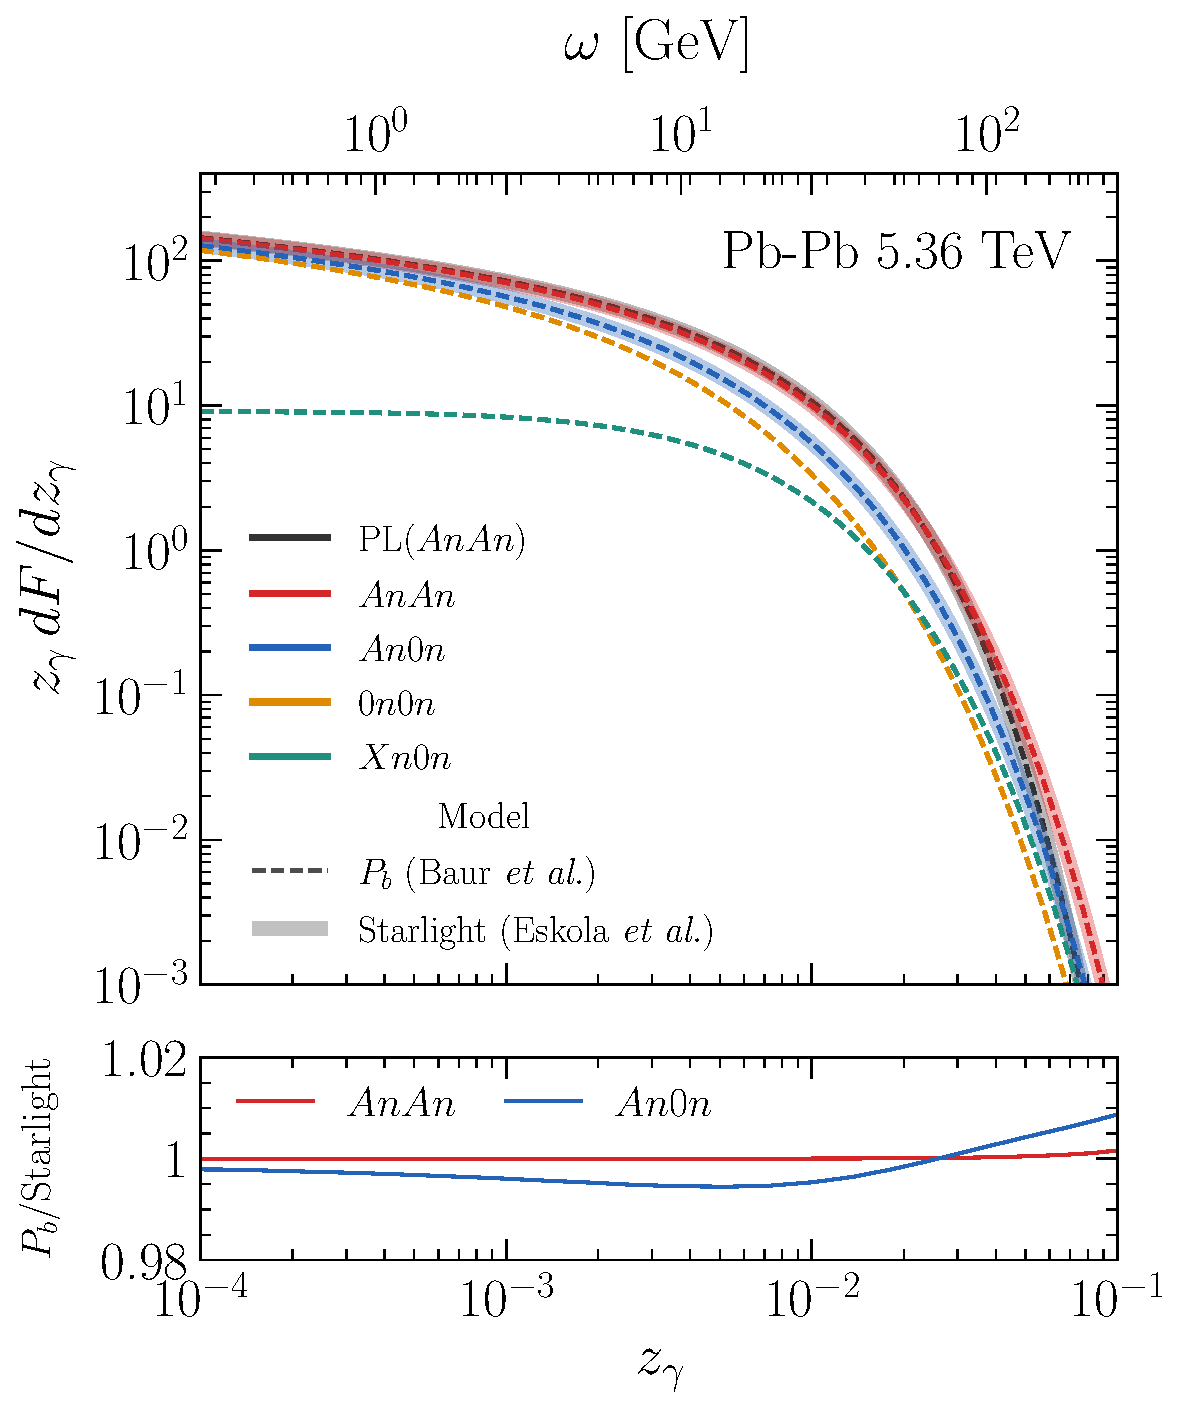
\includegraphics[width=0.8\textwidth]{plots/flux_comparison.pdf}
\caption{This code's simple single-$b$ flux (Eq.~\ref{eq:simple}) vs.\ the
tabulated Starlight flux.}
\label{fig:flux_comparison}
\end{figure}

\begin{figure}[h]
\centering
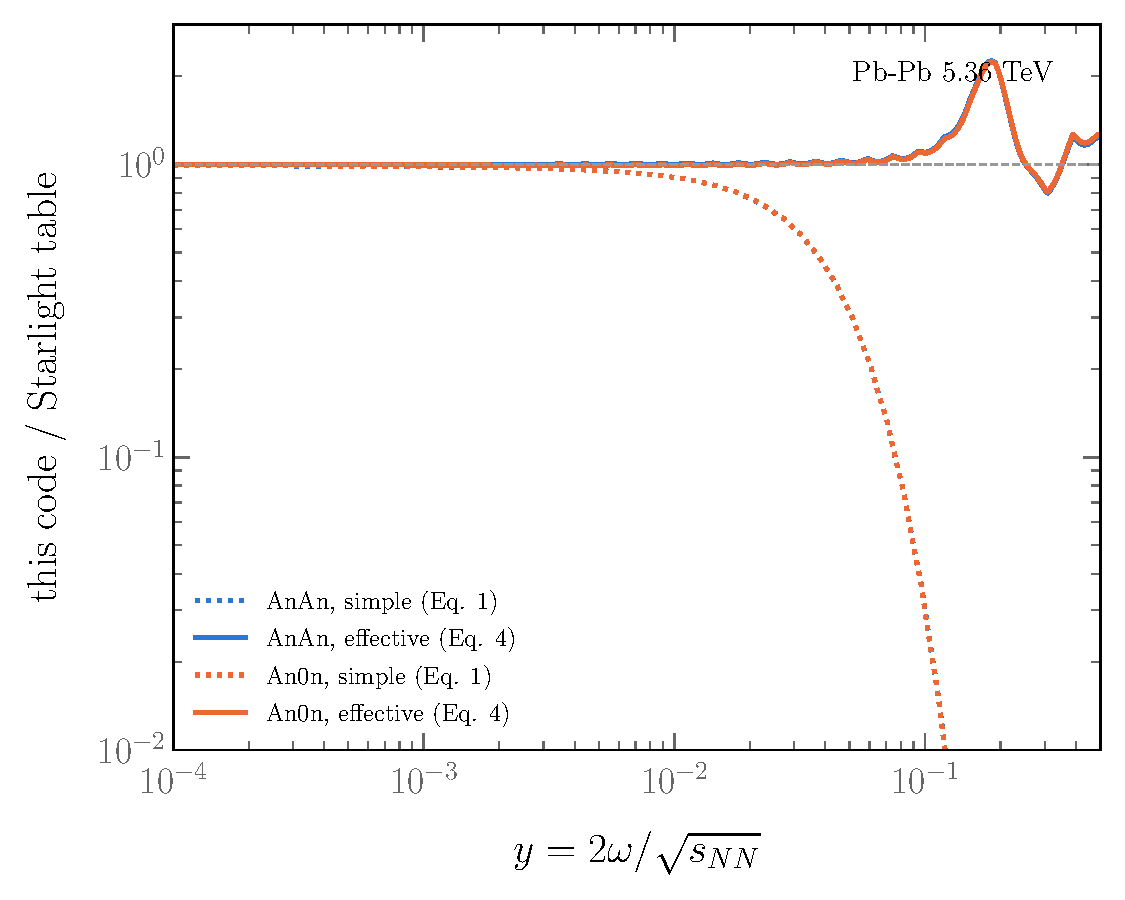
\includegraphics[width=0.8\textwidth]{plots/eff_flux_check.pdf}
\caption{Ratio to the Starlight table: simple (dotted) vs.\ effective-flux
(solid) treatment, for the AnAn and An0n channels.}
\label{fig:eff_check}
\end{figure}

\end{document}
